
\begin{wrapfigure}{r}{0.35\textwidth} \centering
  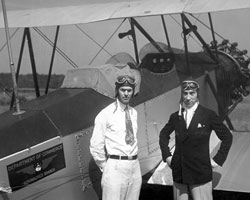
\includegraphics[keepaspectratio,width=0.3\textwidth]{./Imagenes/1931-first-blind-landing.jpg}\caption{Los pilotos James Kinney y Clarence Young con el NS-39 utilizado en las pruebas de vuelo a ciegas. College Park, 1933. \\ \emph{\tiny CPAM Photograph, Kear Collection}} \label{fig:NS-39}
\end{wrapfigure}

Estudios posteriores dieron como resultado el abandono de las se\~nales enclavadas y su reemplazo por tonos de 65 Hz y 87,5 Hz. Despu\'es de ser detectadas por el receptor de la aeronave, ambos tonos se separaban por filtros y las dos se\~nales alimentaban diferencialmente un medidor con el cero en posici\'on central, de esta manera, si el avi\'on se encontraba en el rumbo correcto el medidor indicaba cero, con deflexiones a izquierda o derecha si estaba fuera de rumbo.

Hist\'oricamente, se reconoce como fecha del primer aterrizaje instrumental al 15 de setiembre de 1931. La aeronave NS-39 (Figura \ref{fig:NS-39}),
un Curtiss Fledgling J-1 Special, un biplano de entrenamiento biplaza de cabina abierta ( versi\'on  civil de la aeronave de la marina Curtiss N2C-2),
 lo logr\'o a los mandos de Marshall S. Boggs con James L. Kinney como copiloto en College Park (EE UU).


En 1938 se present\'o un informe que esboz\'o las bases del actual sistema de ILS, las principales recomendaciones eran:

\begin{itemize}
\item El sistema deb\'ia operar en la banda de 180 a 112 Mhz

\item La gu\'ia de la trayectoria vertical deb\'ia ser una l\'inea recta

\item Se deber\'ian instalar dos balizas de distancia que trabajasen a 75 Mhz
\end{itemize}

Posteriormente las frecuencias cambiaron a 90 y 150 Mhz y la frecuencia de gu\'ia vertical a 330 Hz. El resto de los par\'ametros siguieron vigentes hasta nuestros d\'ias, finalizando en el sistema ILS de aterrizaje instrumental.

En 1937 en Estados Unidos se realizaron experiencias utilizando VHF en lugar de MF para los radiofaros omnidireccionales, los resultados fueron prometedores. Se estandariz\'o el uso de frecuencias de 125 Mhz, y tambi\'en se consider\'o el desarrollo de un radiofaro de rumbos infinitos. Esto consisti\'o en un retorno al radiofaro giratorio de Marconi.

El radiofaro resultante empleaba un sistema en el que el diagrama polar horizontal ten\'ia forma de carioide, con la propiedad de que al girar, la intensidad de la se\~nal en cualquier direcci\'on receptora variaba sinusoidalmente. El diagrama giraba a 60 Hz, la onda sinusoidal recibida era separada en dos partes en cuadratura de fase, que eran conectadas a las placas de deflexi\'on de un tubo de rayos cat\'odicos. Esto produc\'ia una traza circular, cada punto de la cual estaba asociado con el instante correspondiente a alguna orientaci\'on particular del diagrama espacial, pero sin ning\'un punto de referencia. Este fue suministrado al principio produciendo una discontinuidad en la se\~nal cuando el m\'aximo del diagrama giratorio pasaba por el norte verdadero, siendo el resultado una deflexi\'on radial en la traza que, de otro modo, ser\'ia circular, proporcionando as\'i una indicaci\'on del rumbo.

En los primeros trabajos sobre dicho radiofaro se utilizaba una frecuencia de 6,5 Mhz, pero en vista de la tendencia en favor del VHF se pas\'o a la de 125 Mhz.

En el receptor se comparaban las fases de la se\~nal de referencia y la se\~nal giratoria, correspondiendo la diferencia de fase con el rumbo del receptor. Debido a esta modificaci\'on en la se\~nal de referencia se dej\'o de usar como indicador el tubo de rayos cat\'odicos, que fue sustituido por un medidor de fase con indicaci\'on azimutal.
